
\chapter{Results} 

\label{Chapter5}

%----------------------------------------------------------------------------------------

In this chapter we discuss the results obtained in this thesis. First, we analyze how the model works for a few given resolutions, so that we can be confident about its performance. Then, we consider how the accuracy changes with the resolution and within the categories. Finally, we discuss the cost around Satellite imagery to analyze once the entire earth. 

\section{Transfer learning on aerial imagery}

The first thing we want to investigate from our experiments is whether the approach followed is able to achieve good results. That is, we want to evaluate if using a pre-trained ResNet as a feature extractor for aerial images allows the trained model to properly discriminate the existence of human impact. 

Tables \ref{tab:Results_03m_100n} - \ref{tab:Results_1m_200n} in Appendix \ref{Tables} show that the accuracies obtained with all the experiments are indeed remarkable. All these results are discussed in more detail in the next section, but let us begin by focusing on few cases of the $0.3m$ dataset in order to understand how the models are behaving. In table \ref{tab:Results_03m_100n} we can see that an accuracy of around $0.9226$ is achieved on the base resolution ($0.3m$), while it drops to $0.8690$ of the last downgraded resolution of the dataset ($4.8m$).

Let us consider first some examples of correctly and wrongly classified images at the base resolution (for one of the cross-validation folds), which are shown in Figures \ref{fig:dataset03m_res03_correct} and \ref{fig:dataset03m_res03_wrong} respectively. The first set of samples shows that the model accurately detects clear human impact related to agriculture (2nd picture in the second row) and paths. On the other hand, the second set shows that it might fail to detect it when the impact is subtle, covering a small region of the image, or when it can even be confused with natural structures (or vice versa).

Note that, from this point, \textit{label 1} refers to images with clear human impact, which were defined as \textit{label 2} when building the datasets in Chapter \ref{Chapter2}.

\begin{figure}[H]
	\centering
	\captionsetup{width=1\linewidth}
	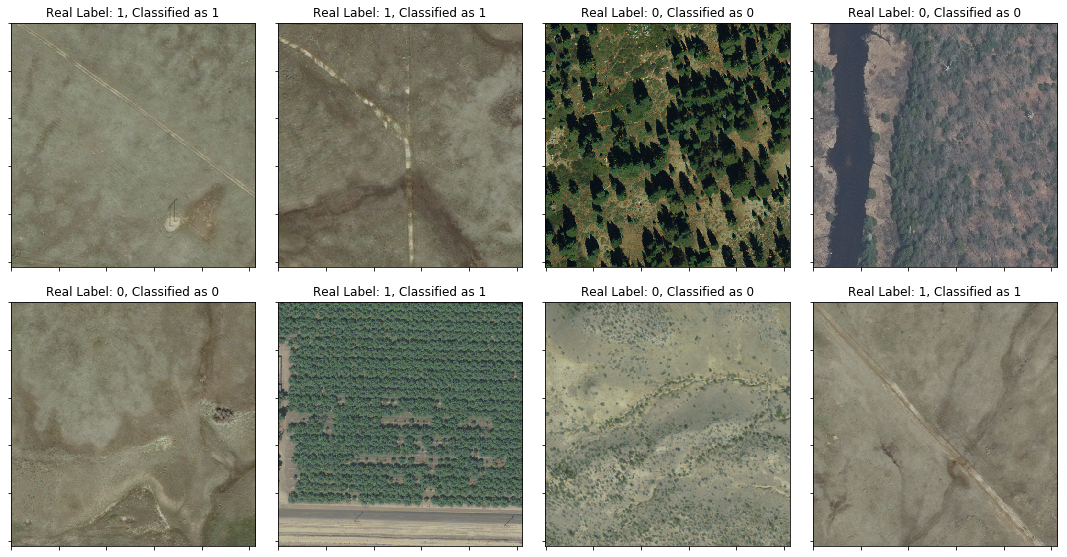
\includegraphics[width=1\textwidth]{Figures/results/class_dataset03m_res03_correct.png}
	\caption{\textbf{Examples of correctly classified images at the base resolution, $0.3m$.}}
	\label{fig:dataset03m_res03_correct}
\end{figure}

\begin{figure}[H]
	\centering
	\captionsetup{width=1\linewidth}
	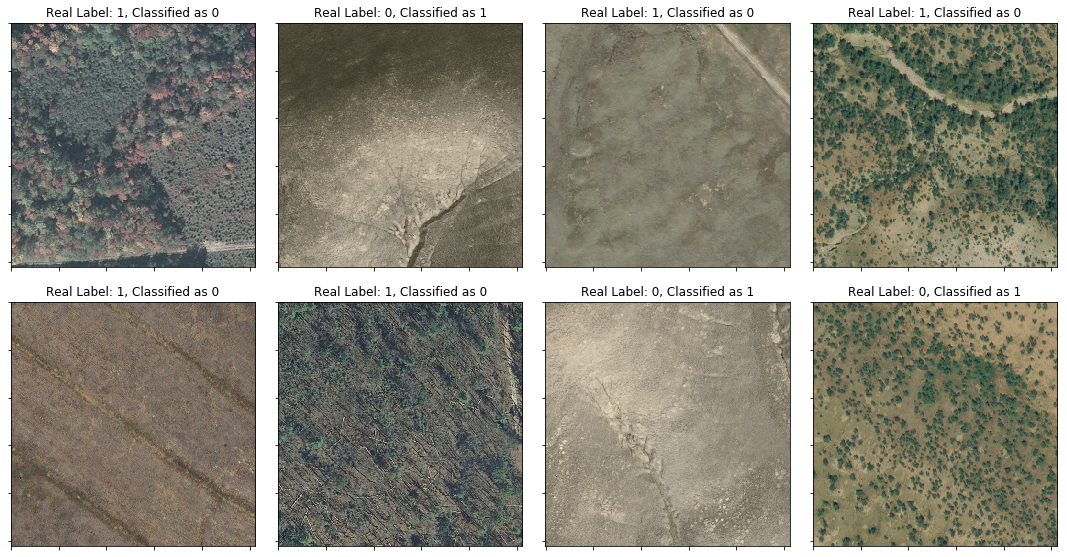
\includegraphics[width=1\textwidth]{Figures/results/class_dataset03m_res03_wrong.png}
	\caption{\textbf{Examples of wrongly classified images at the base resolution,  $0.3m$.}}
	\label{fig:dataset03m_res03_wrong}
\end{figure}

The same kind of analysis can be done for the last resolution, $4.8m$. Figures \ref{fig:dataset03m_res48_correct} and \ref{fig:dataset03m_res48_wrong} show correctly and wrongly classified images at this resolution. The first set shows that the model detects human impact when it is still evident, even with the low resolution, but the second set indicates that it commits mistakes when the human impact evidences are lost with the downgrade process. Similarly, it might classify as man-made structures patterns that are indeed natural.

\begin{figure}[H]
	\centering
	\captionsetup{width=1\linewidth}
	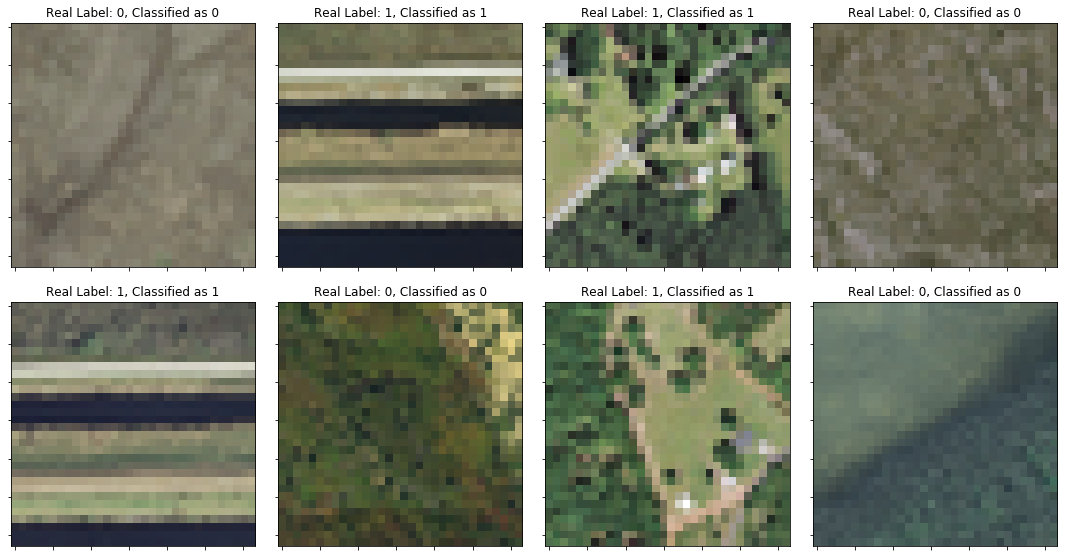
\includegraphics[width=1\textwidth]{Figures/results/class_dataset03m_res48_correct.png}
	\caption{\textbf{Examples of correctly classified images at the last resolution, $4.8m$.}}
	\label{fig:dataset03m_res48_correct}
\end{figure}

\begin{figure}[H]
	\centering
	\captionsetup{width=1\linewidth}
	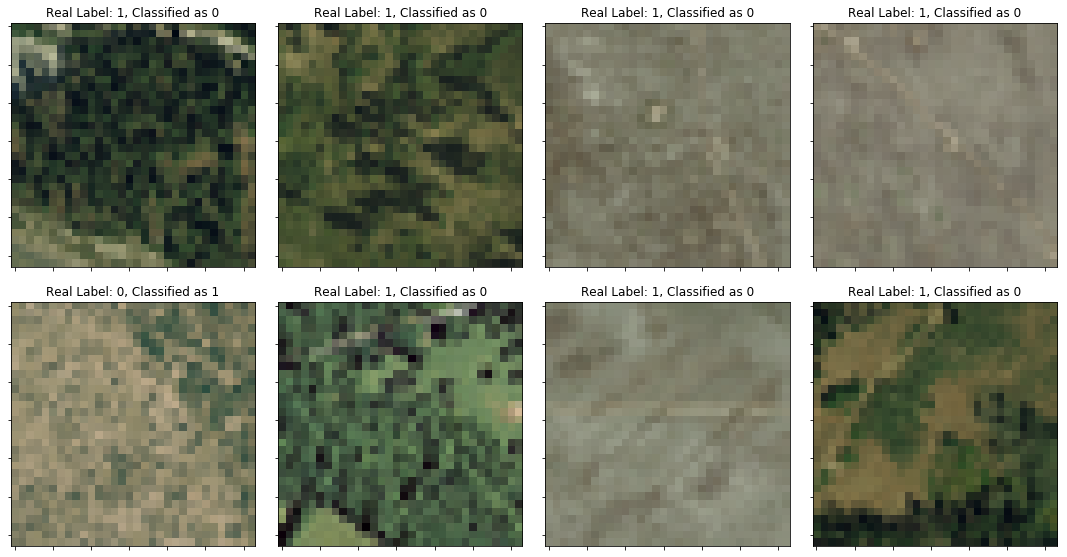
\includegraphics[width=1\textwidth]{Figures/results/class_dataset03m_res48_wrong.png}
	\caption{\textbf{Examples of wrongly classified images at the last resolution, $4.8m$.}}
	\label{fig:dataset03m_res48_wrong}
\end{figure}

This can also be seen with Figure \ref{fig:dataset03m_res03_res48_comp}, which shows images that are correctly classified at $0.3m$ resolution (top row) but wrongly classified at $4.8m$. The first and third pair of images demonstrate that, when the human impact is subtle, the model missed it in the downgraded resolution. Conversely, non human activity can also be misclassified at lower resolutions (second and fourth images).

\begin{figure}[H]
	\centering
	\captionsetup{width=1\linewidth}
	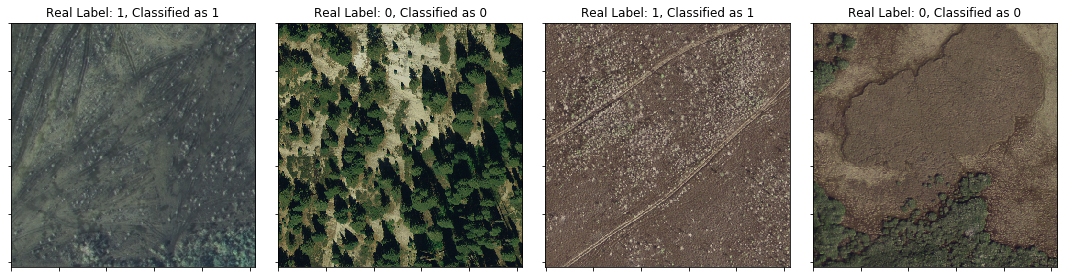
\includegraphics[width=1\textwidth]{Figures/results/class_dataset03m_res03_comp_correct.png}
	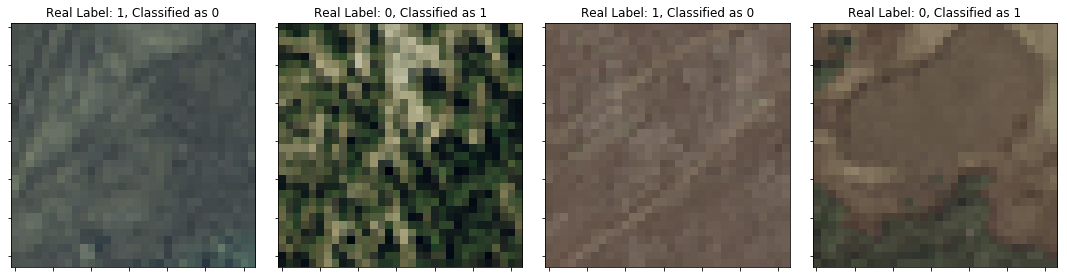
\includegraphics[width=1\textwidth]{Figures/results/class_dataset03m_res48_comp_wrong.png}
	\caption{\textbf{Correctly and wrongly classified images at different resolutions.} Here the first row displays images in their base resolution, $0.3m$. These images were correctly classified by the model. The same images at a resolution of $4.8m$ (second row) were wrongly classified by the model.}
	\label{fig:dataset03m_res03_res48_comp}
\end{figure}

Finally, we can investigate how the model behaves with images where human impact is very subtle. For this purpose, we consider the images with the intermediate label (\textit{label 1} in Chapter \ref{Chapter2}, Figure \ref{fig:imstats}). The model has never been faced with these images, so this can give a good perception of whether the models have been able to learn relevant features of human impact. Figure \ref{fig:dataset03m_res03_l1} shows some of these images with the label predicted by the model in the title. Even if man-made structures in these pictures are small, the model is able to detect straight lines and shapes as human activity. 

\begin{figure}[H]
	\centering
	\captionsetup{width=1\linewidth}
	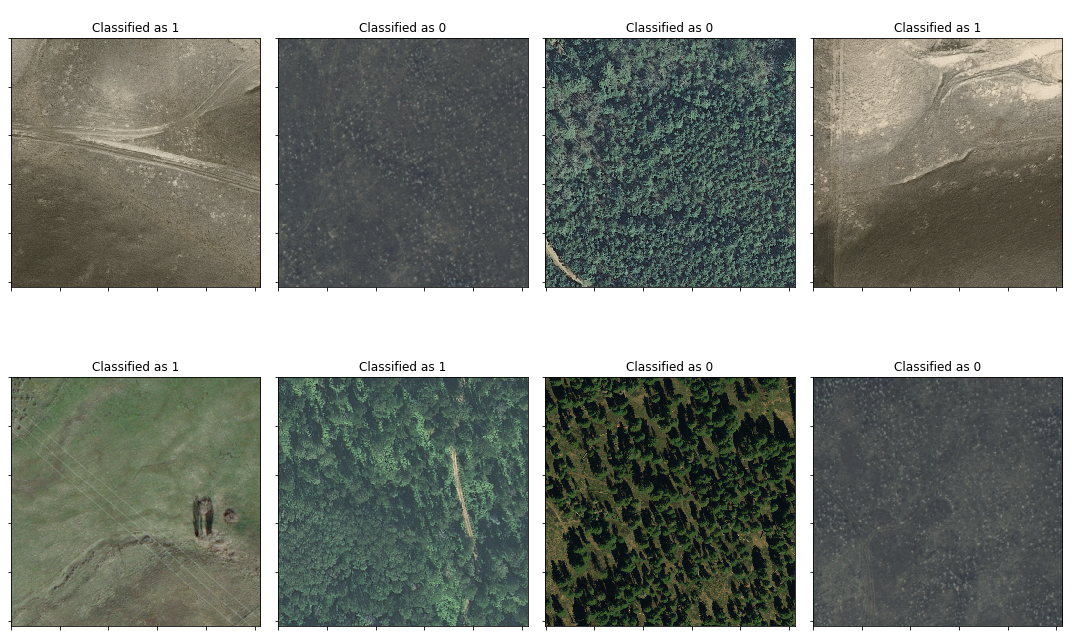
\includegraphics[width=1\textwidth]{Figures/results/class_dataset03m_res03_l1.png}
	\caption{\textbf{Examples of predictions made for images with subtle human impact}. Images showing minimal human impact were referred to as label 1 images in Chapter \ref{Chapter2}. Note that these images were not used when training the model.}
	\label{fig:dataset03m_res03_l1}
\end{figure}

All in all, we can conclude that the model is able to achieve a great accuracy. It is able to generalize to unseen, subtle images, and still be accurate for lower resolutions, were the amount of pixels and information per images become much smaller. 

\section{Man-made structures detection at different scale}

Now that we know that the trained models are able to detect, with high accuracy, human impact from our datasets, we are ready to analyze the results for different resolutions. From all the experiments (datasets, architectures, resolutions and cross-validations), the results have been stored and aggregated. As mentioned in the previous chapter, the models were not able to converge for some particular splits of the datasets. Hence, these few folds have been ignored when aggregating the results. Tables \ref{tab:Results_03m_100n} - \ref{tab:Results_1m_200n} in Appendix \ref{Tables} summarize the accuracies obtained for each of the datasets ($0.3m$ and $1m$) and downgraded resolutions, both the overall accuracy and by category. 

Similarly, Figure \ref{fig:acc_res_03m_1m} shows the overall accuracies obtained for all resolutions. From this we can see that similar accuracies are achieved for both datasets on the same degraded resolution, which means that both datasets are comparable and can be considered together. Also, we realize that increasing the size of the model from $100$ neurons to $200$ does not have a big impact on the accuracy, but tends to perform slightly better. Hence, for other results later we will focus on this architecture only.

\begin{figure}[h!]
	\centering
	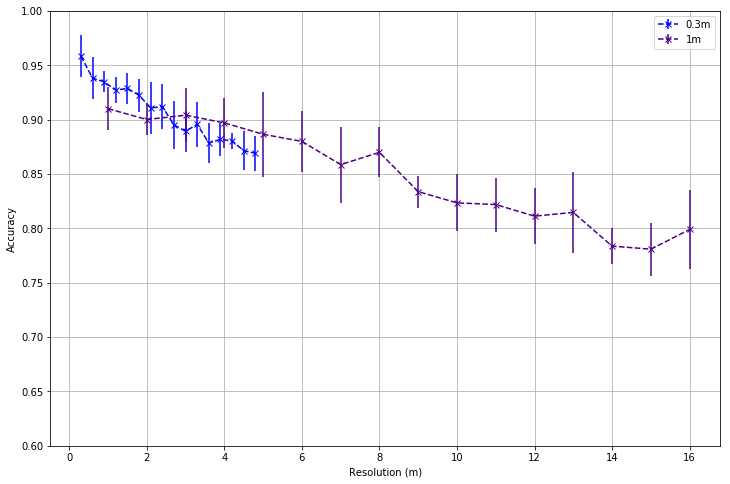
\includegraphics[width=0.8\textwidth]{Figures/results/acc_res_03m_1m.png}
	\captionsetup{width=1\linewidth}
	\caption{\textbf{Accuracy at each resolution for all datasets and architectures.} Similar results are obtained at the same degraded resolutions. The vertical lines represent the variability (standard deviation) for the different folds of the cross-validations.}
	\label{fig:acc_res_03m_1m}
\end{figure}

On closer inspection, we also detect that the accuracy on the base resolution ($0.3m$ and $1m$) is always slightly worse than the next resolution. This is probably because the input image size at the base resolution is quite large ($512\times512$), which makes the dense layer much more complex to train. Indeed, Figures \ref{fig:conv_plots_03m} and \ref{fig:conv_plots_1m} in Chapter \ref{Chapter4} already suggest that the models struggle to be optimized. Additionally, when training for the $0.3m$ resolution, we had to consider a smaller subset of images (around $1500$ instead of $2000$), as the Google Colab instance we were using could not load all the data in memory. This might also have had an impact on the accuracy obtained, yet it seems to be consistent with the results for the $1m$ resolution, were the whole dataset was considered. All in all, having a more powerful computer capable of dealing with more sample images could help to compensate for the complexity and achieve a greater accuracy. 

Finally, the overall conclusion from this plot is that, as expected, better resolutions (less than $2m$) allow for greater accuracies, of over $90\%$, which means a great success considering that the images in the datasets are balanced between having or not human impact. Furthermore, accuracy is still good for resolutions between $2m$ and $8m$, staying between $85\%$ and $90\%$. From $8m$ onwards, accuracy drops to $80\%$ and the model is not able to detect more subtle elements of man-made structures.

Now let us consider how these accuracies behave for each of the land use categories in the datasets. As discussed in section \ref{usgs_data}, these categories are rough approximations of the kind of terrain and human impact, with images that could be exchanged between categories, but overall these can give and idea of the accuracies when analyzing different kind of terrains. Indeed, Figures \ref{fig:acc_all_cat_03m} and \ref{fig:acc_by_cat_03m} show that, for the $0.3m$ dataset (and $200$ neurons model), accuracy differs substantially between categories. Fig. \ref{fig:acc_all_cat_03m} shows the global comparison between categories, while Fig. \ref{fig:acc_by_cat_03m} allows for a better comparison of each category with respect to the overall accuracy. 

\begin{figure}[h!]
	\centering
	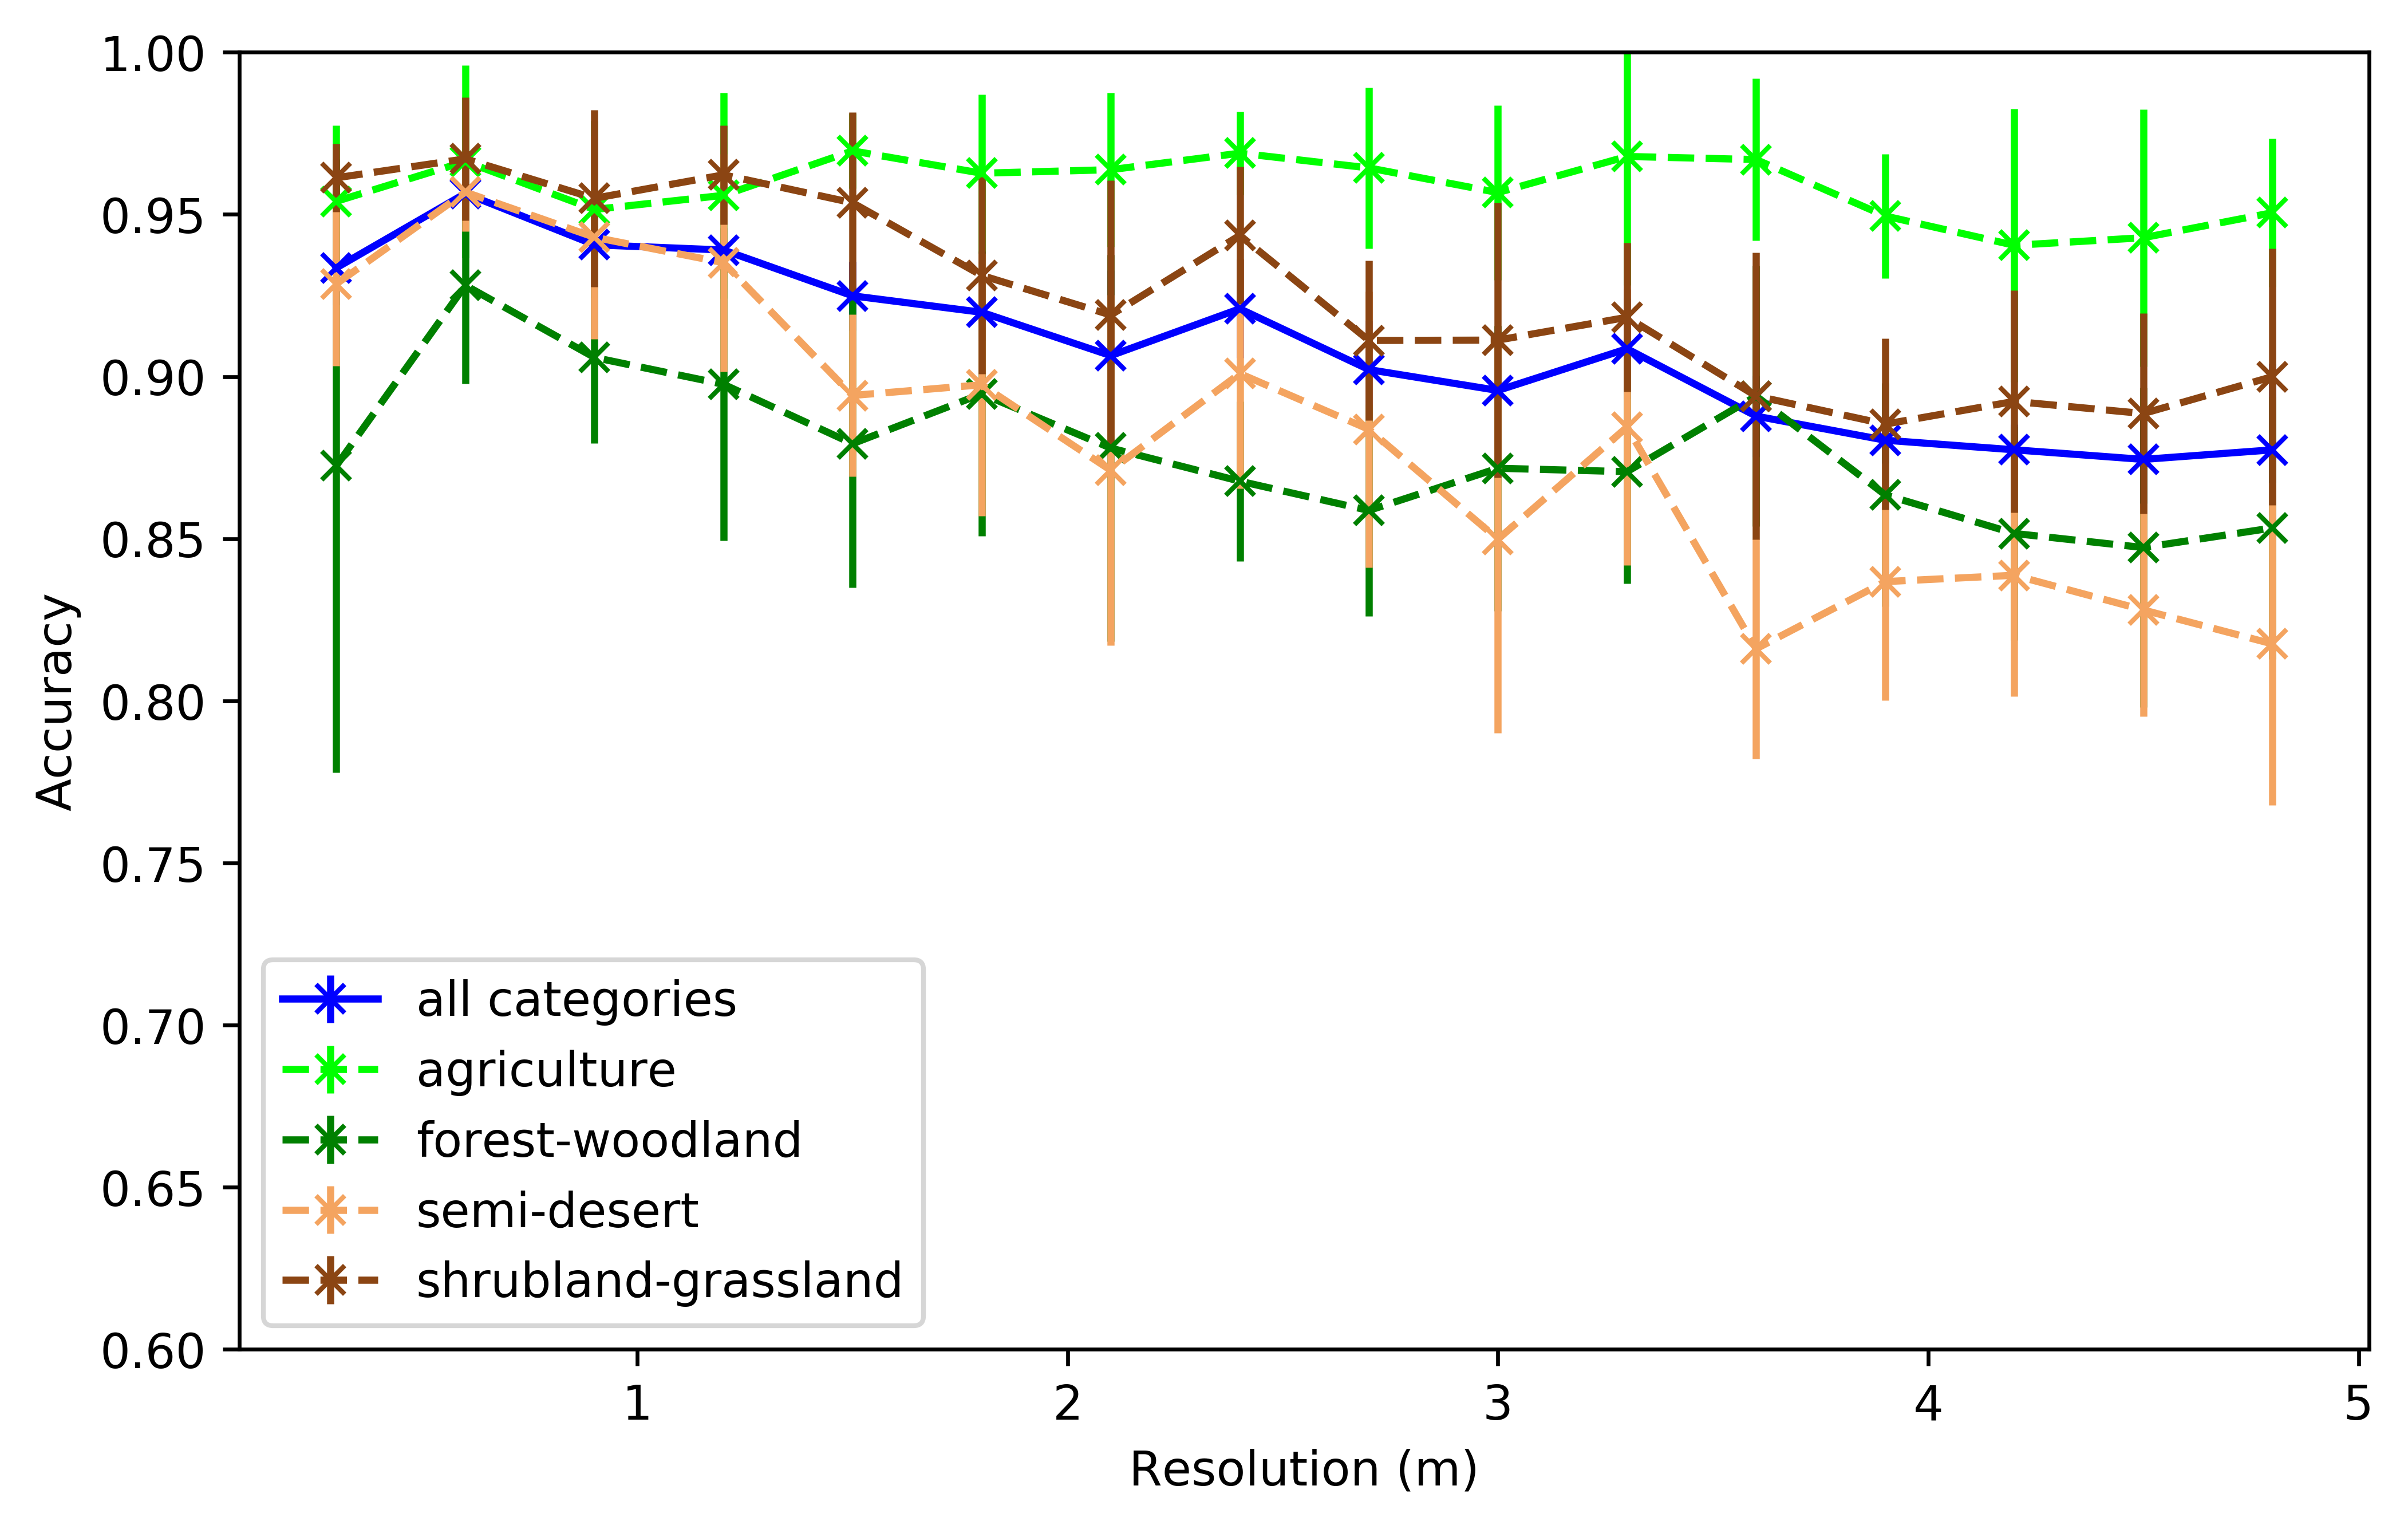
\includegraphics[width=0.8\textwidth]{Figures/results/acc_res_all_categories_03m.png}
	\captionsetup{width=1\linewidth}
	\caption{\textbf{Accuracies obtained for each category, with the model trained over all categories, on the $0.3m$ dataset.}}
	\label{fig:acc_all_cat_03m}
\end{figure}

\begin{figure}[h!]
	\centering
	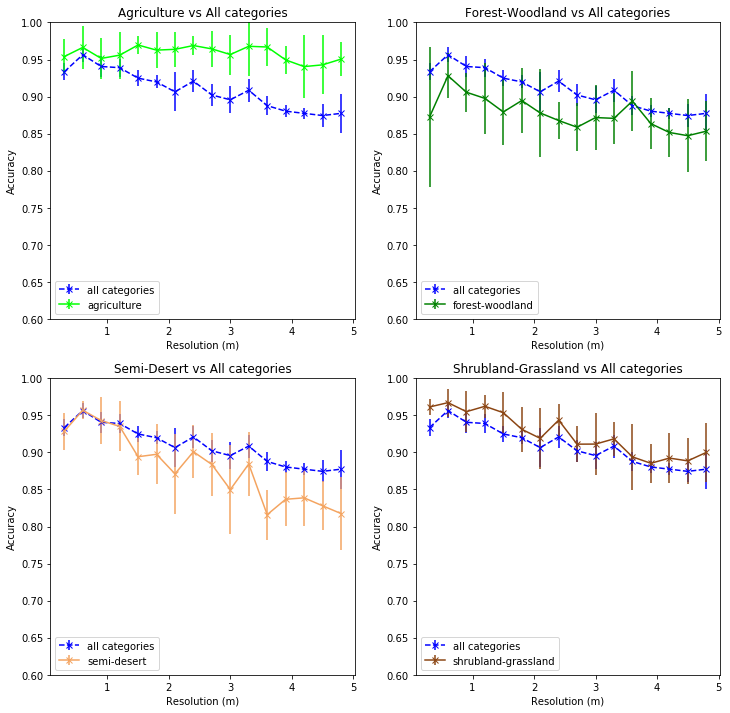
\includegraphics[width=0.9\textwidth]{Figures/results/acc_res_by_category_03m.png}
	\captionsetup{width=1\linewidth}
	\caption{\textbf{Comparsion of accuracies between each category and overall, with the model trained over all categories, on the $0.3m$ dataset.}}
	\label{fig:acc_by_cat_03m}
\end{figure}

These plots have been obtained once the model was trained for all the categories. Then, the accuracy on the validation set was computed for each individual category and over all images in the set. The validation set in each iteration of the cross-validation was small, consisting of few hundred images, and a homogeneous representation of the categories was not imposed (validation samples were picked randomly, only preserving proportion between having or not human impact), which explains the large variability for each experiment (vertical lines in the plots).

Although the category is not taken into account when training, we can see that the models are capable of detecting agriculture-related human impact with high accuracy (over $95\%$), without really being affected by the drop in accuracy. Shrubland-grassland category also has a good accuracy, while the model performs worse in semi-desert and forest-woodland images. That means that the models are able to capture textures and patterns related to agriculture quite easily, while the other categories have more variable features.

Similar results are obtained for the $1m$ dataset, which are shown in Figures \ref{fig:acc_all_cat_1m} and \ref{fig:acc_by_cat_1m}. The models are able to achieve a great accuracy when detecting agriculture-related human impact (over $95\%$), independently of the resolution considered, but the performance drops for the other 3 categories. The biggest drop is observed at $8m$ consistently over the three non-agriculture categories. 

\begin{figure}[H]
	\centering
	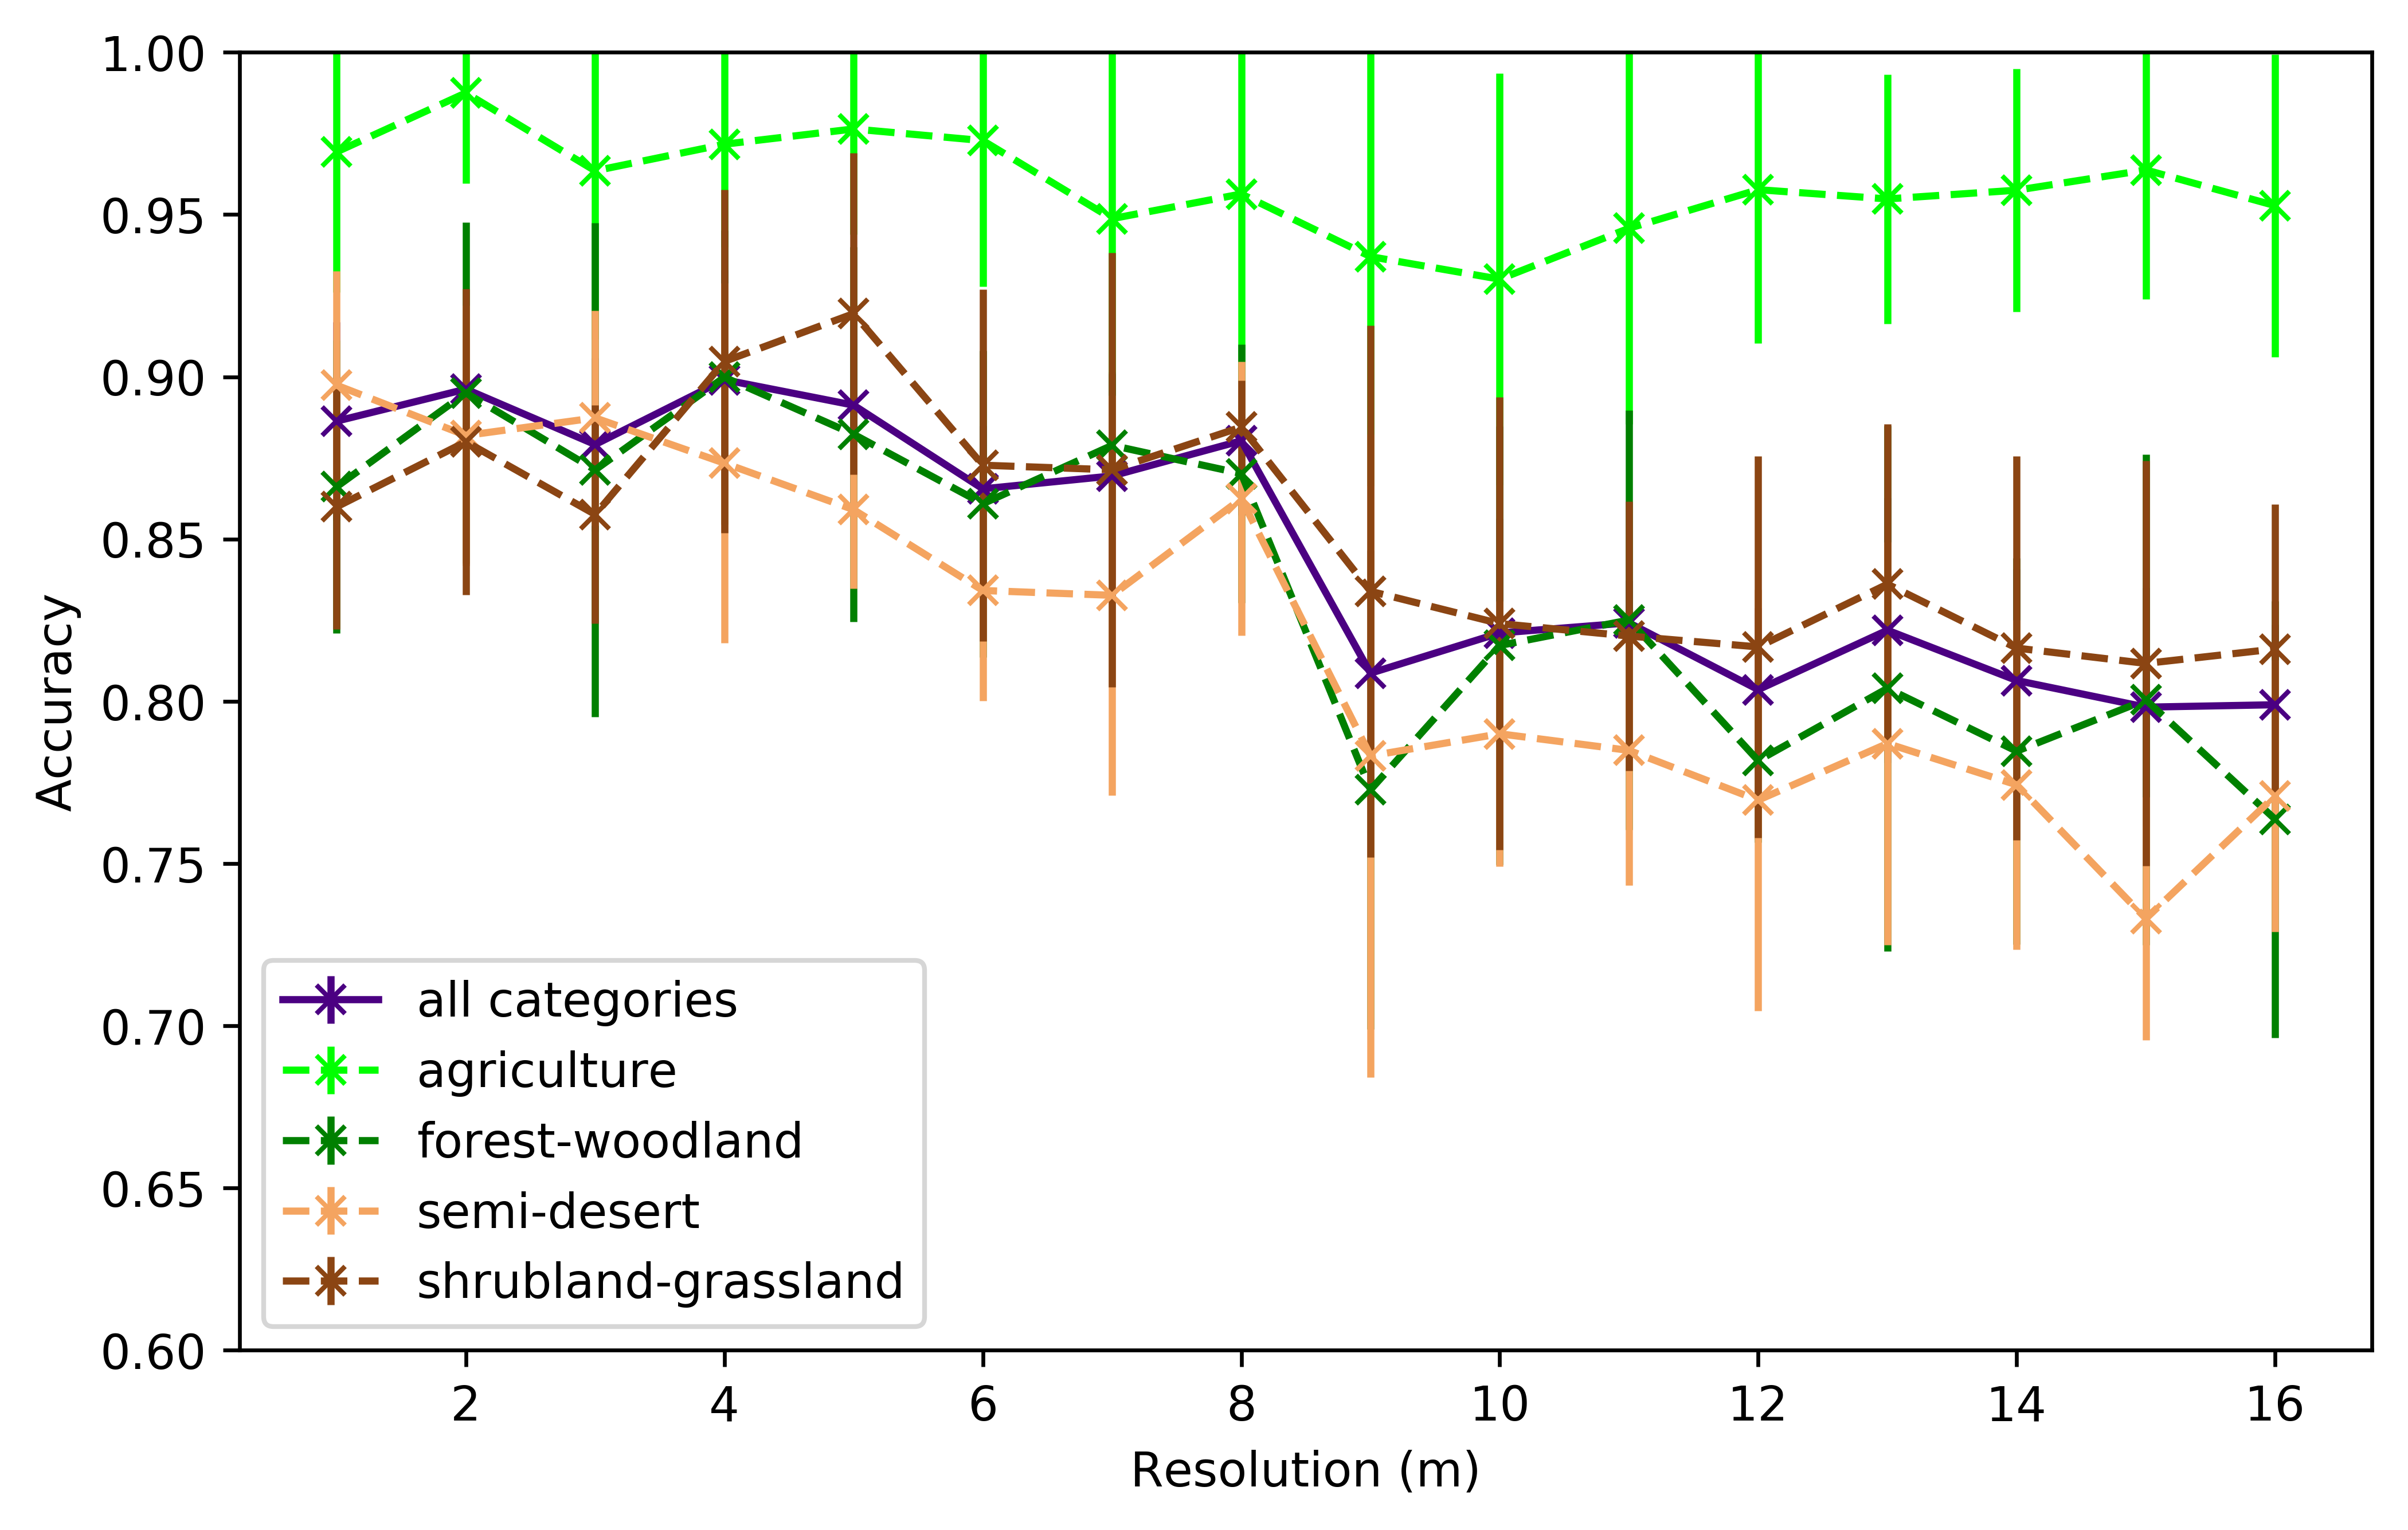
\includegraphics[width=0.8\textwidth]{Figures/results/acc_res_all_categories_1m.png}
	\captionsetup{width=1\linewidth}
	\caption{\textbf{Accuracies obtained for each category, with the model trained over all categories, on the $1m$ dataset.}}
	\label{fig:acc_all_cat_1m}
\end{figure}

\begin{figure}[H]
	\centering
	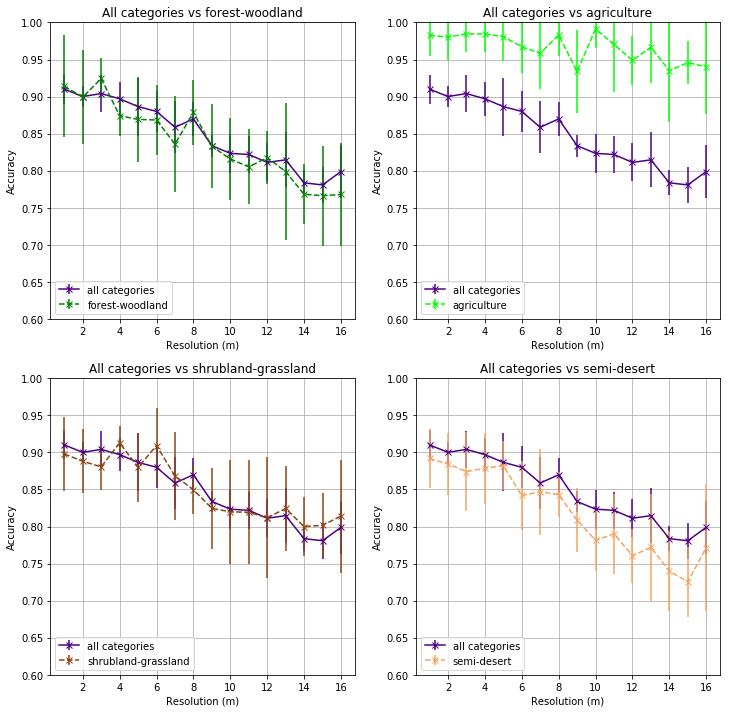
\includegraphics[width=0.9\textwidth]{Figures/results/acc_res_by_category_1m.png}
	\captionsetup{width=1\linewidth}
	\caption{\textbf{Comparsion of accuracies between each category and overall, with the model trained over all categories, on the $1m$ dataset.}}
	\label{fig:acc_by_cat_1m}
\end{figure}


\section{Cost estimation}

We discuss the financial cost associated to building and launching a satellite, and to renting infrastructure for performing the entire image processing pipeline. We further study the cost as a function of pixel resolution. However, our estimates are very rough approximations because many factors are involved and large variations occur between them. To give an example, choosing one material over the other might change the cost of manufacturing and launching a satellite by one order of magnitude. It is also completely different to have a satellite for 3 years in space, or to target a lifespan of 20 years. 

Having this in mind, we follow laws from physics to estimate the dependency of the satellite cost on resolution. First, the cost of launching a satellite into the orbit scales linearly with its mass \parencite{rocket_equation}, which is given by the amount of fuel needed. Second, the mass of the satellite scales quadratic with resolution so that overall we obtain a cubic dependency for launching a satellite into space. The latter increase in cost is associated with the optical instruments used. As a reference for the satellite cost we use a Skysat satellite from Planet \parencite{skysat_planet} that has a resolution of about 1m and a value of $\$30$ million. This amount was provided to us by Satellogic and includes construction, launch and maintenance during the satellite's lifespan.

Our final goal is to give an estimation of the expenditure to monitor once the entire surface of the earth (about 149 million km$^2$). To this end, we multiply the satellite cost by the ratio: time needed to scan the earth over the satellite's lifespan. Further, a satellite can map 1 million km$^2$ at 1m resolution in 4.2 days \parencite{satellogic_youtube}. We hence can calculate the satellite cost per km$^2$. Assuming a lifespane of 10 years we have $area = 10^6 \times \frac{10\cdot365}{4.2}~km^2$ so we obtain $cost~satellite~per~km^2 = cost~satellite/area \approx 0.035~\$/km^2$.

\begin{table}[h!]
	\begin{tabular}{l | l | l | l | l}
		description & cost & unit & cost (\$/km$^2$) & cost (\$/pixel) \\
		\hline
		process raw data & & & 0.004 & $4 \times 10^{-9}$ \\
		hot storage  & $72\times 10^{-6}$ & \$/(km$^2$/month) & 0.000864 & $8.64\times10^{-10}$ \\
		cold storage  & $36\times 10^{-6}$ & \$/(km$^2$/month) & 0.000432 & $4.32\times10^{-10}$ \\
		archive storage  & $9\times 10^{-6}$ & \$/(km$^2$/month) & 0.000108 & $1.08\times10^{-10}$ \\
		download data & 8 & \$/Gb & 0.021 & $2.1  \times 10^{-8}$\\
		serving to final client & 0.09 & \$/Gb & 0.000236 & $4.7232 \times 10^{-10}$\\
		prediction (AWS) & 0.05 \& $\sim$6 & \$/h \& s/km$^2$ & 0.00145 & $1.45 \times 10^{-9}$\\
	\end{tabular}
	\captionsetup{width=1\linewidth}
	\caption{\textbf{Costs for image data processing.} All costs except the prediction are provided by Satellogic.}
	\label{table:data_costs}	
\end{table}

Another cost intensive block when capturing satellite imagery involves image data processing for which the cost scales quadratic with resolution. For example, an operation that costs 100\$/km$2$ at 1m resolution will cost only 1\$/km$^2$ at 10m resolution. The data processing step consists of multiple parts: transformation of raw data into image pixels, storing data in a hot, cold, and archive storage, downloading data from the satellite, serving it to the final client, and in our case predicting human impact. These costs are summarized for 1m resolution in table \ref{table:data_costs}. Note that we used the conversion factor 0.002624 for an image to convert from Gigabytes to km$^2$ (2$\times$ compressed) and we assume 12 months of data storage. 

The prediction step is estimated by loading 4 images that each have an area of about $500\times500m^2$, calculating the ResNet activations of the final layer, and predicting the class using the models trained in chapter~\ref{Chapter4} in an ensemble fashion. This part amounts to a processing time of about 6s for an area of 1km$^2$, which can be converted into costs per km$^2$ assuming 0.05\$/h of AWS EC2 compute~\parencite{aws}.

To finally obtain the dependence of the resolution on the total financial cost we sum the data cost per km$^2$ and the satellite cost per km$^2$ at 1m resolution, and convert to cost per pixel ($\times 10^{-6}$). We then multiply with the number of pixels necessary to cover the entire surface of the earth. Here the satellite cost per km$^2$ is a cubic function and the earth surface in pixel is a quadratic function in resolution. The result is shown in Fig.~\ref{fig:costs}. We obtain a cost of about \$15 million dollars at 1m resolution with a very steep slope towards better resolutions. At 0.3m resolution the cost is two orders of magnitude higher than at 1m while for worse resolutions the cost decreases by two orders of magninute when the resolution is about 10m. We conclude that for worse resolutions the data processing cost is the dominating cost whereas for very good resolutions the satellite cost dominates.

\begin{figure}[h!]
	\centering
	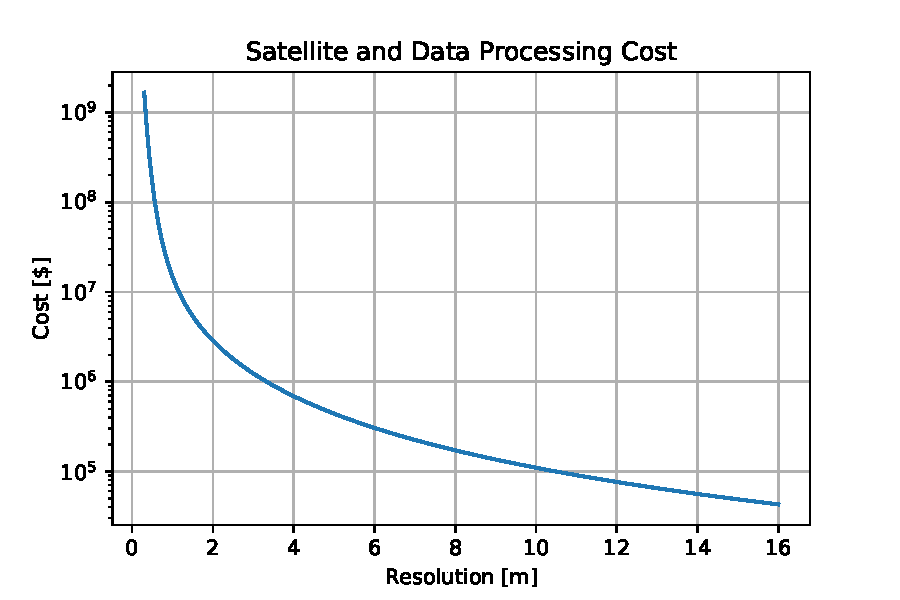
\includegraphics[width=0.75\textwidth]{Figures/costs.pdf}
	\captionsetup{width=1\linewidth}
	\caption{\textbf{Satellite and data processing cost.} The total financial cost to capture images with a satellite and process the data as function of resolution.}
	\label{fig:costs}
\end{figure}


